\documentclass[10pt]{article}
\usepackage{color}
\usepackage{tikz}


\newcommand{\indep}{\rotatebox[origin=c]{90}{$\models$}}

% https://dkumor.com/posts/technical/2018/08/15/causal-tikz/

% Tikz settings optimized for causal graphs.
% Just copy-paste this part
\usetikzlibrary{shapes,decorations,arrows,calc,arrows.meta,fit,positioning}
\tikzset{
    -Latex,auto,node distance =1 cm and 1 cm,semithick,
    state/.style ={ellipse, draw, minimum width = 0.7 cm},
    point/.style = {circle, draw, inner sep=0.04cm,fill,node contents={}},
    bidirected/.style={Latex-Latex,dashed},
    el/.style = {inner sep=2pt, align=left, sloped}
}
\begin{document}



  
  %%%%%%% 2st 

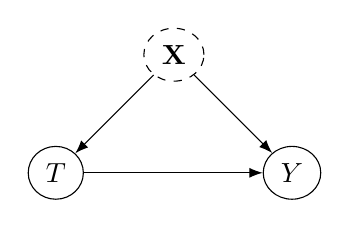
\begin{tikzpicture}
    \node[state, dashed] (i) at (0,0) {$\mathbf{X}$};
      \node[state] (t) at (-1.5,-1.5) {$T$};
       \node[state] (y) at (1.5, -1.5) {$Y$};
     
      \path (t) edge (y);
       \path (i) edge (t);
        \path (i) edge (y);
  

\end{tikzpicture}


  \clearpage
  
%%%%%%% 1st 

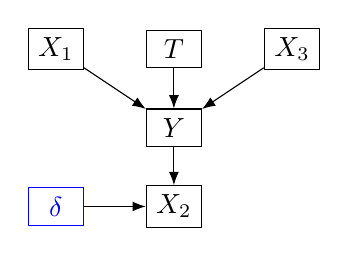
\begin{tikzpicture}
    \node[state, rectangle] (y) at (0,0) {$Y$};
    \node[state, rectangle] (x1) at (-1.5,1) {$X_1$};
     \node[state, rectangle] (x3) at (1.5,1) {$X_3$};
    \node[state, rectangle] (x2) at (0,-1) {$X_2$};
    \node[state, rectangle] (t) at (0,1) {$T$};
     \node[state, blue, rectangle] (d) at (-1.5,-1) {$\delta$};
    
    \path (t) edge (y);
    \path (x1) edge (y);
     \path (x3) edge (y);
     \path (y) edge (x2);     
        \path (d) edge (x2);     
       
\end{tikzpicture}
  
  \clearpage
  
  


%%%%%%% 1st 

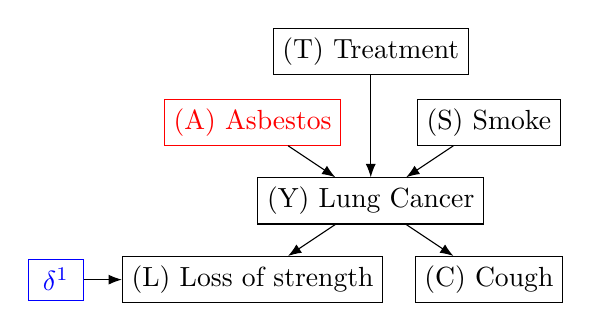
\begin{tikzpicture}
    \node[state, rectangle] (y) at (0,0) {(Y) Lung Cancer};
    \node[state, red, rectangle] (x1) at (-1.5,1) {(A) Asbestos};
    \node[state, rectangle] (x2) at (-1.5,-1) {(L) Loss of strength};
    \node[state, rectangle] (x4) at (1.5,1) {(S) Smoke};
    \node[state, rectangle] (x3) at (1.5,-1) {(C) Cough};
    \node[state, rectangle] (t) at (0,1.9) {(T) Treatment};
     \node[state, blue, rectangle] (d) at (-4,-1) {$\delta^1$};
    
    \path (t) edge (y);
    \path (x1) edge (y);
     \path (x4) edge (y);
     \path (y) edge (x2);     
    \path (y) edge (x3);   
        \path (d) edge (x2);     
       
\end{tikzpicture}
  
  \clearpage
  
  
  
 
%%%%%%% 1st 


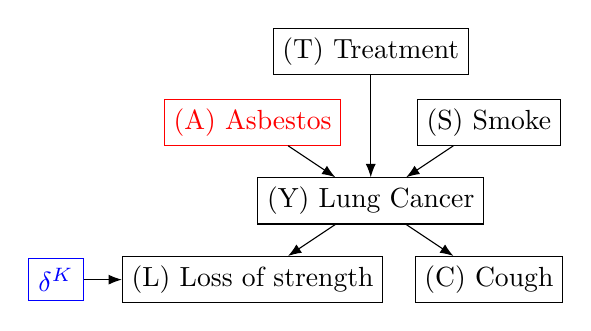
\begin{tikzpicture}
 \node[state, rectangle] (y) at (0,0) {(Y) Lung Cancer};
    \node[state, red, rectangle] (x1) at (-1.5,1) {(A) Asbestos};
    \node[state, rectangle] (x2) at (-1.5,-1) {(L) Loss of strength};
    \node[state, rectangle] (x4) at (1.5,1) {(S) Smoke};
    \node[state, rectangle] (x3) at (1.5,-1) {(C) Cough};
    \node[state, rectangle] (t) at (0,1.9) {(T) Treatment};
     \node[state, blue, rectangle] (d) at (-4,-1) {$\delta^K$};
    
    \path (t) edge (y);
    \path (x1) edge (y);
     \path (x4) edge (y);
     \path (y) edge (x2);     
    \path (y) edge (x3);   
        \path (d) edge (x2);     
       
\end{tikzpicture}
  
  \clearpage
  
  
 
%%%%%%% 1st 


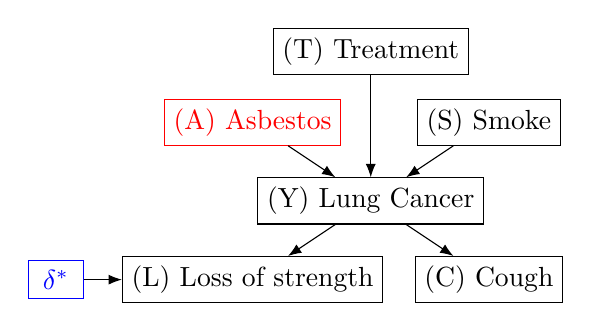
\begin{tikzpicture}
 \node[state, rectangle] (y) at (0,0) {(Y) Lung Cancer};
    \node[state, red, rectangle] (x1) at (-1.5,1) {(A) Asbestos};
    \node[state, rectangle] (x2) at (-1.5,-1) {(L) Loss of strength};
    \node[state, rectangle] (x4) at (1.5,1) {(S) Smoke};
    \node[state, rectangle] (x3) at (1.5,-1) {(C) Cough};
    \node[state, rectangle] (t) at (0,1.9) {(T) Treatment};

     \node[state, blue, rectangle] (d) at (-4,-1) {$\delta^{*}$};
    
    \path (t) edge (y);
    \path (x1) edge (y);
     \path (x4) edge (y);
     \path (y) edge (x2);     
    \path (y) edge (x3);   
        \path (d) edge (x2);     
       
\end{tikzpicture}
  
  \clearpage


  
  
  %%%%%%% 2st 

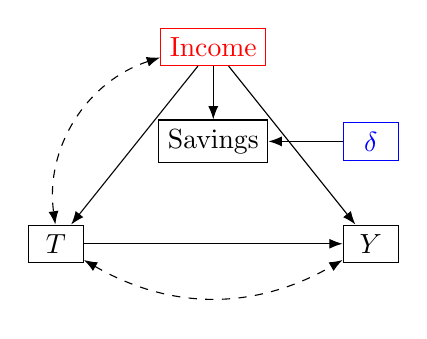
\begin{tikzpicture}
    \node[state, red, rectangle] (i) at (0,0) {Income};
     \node[state, rectangle] (s) at (0,-1.2) {Savings};
       \node[state, blue, rectangle] (d) at (2,-1.2) {$\delta$};
      \node[state, rectangle] (t) at (-2,-2.5) {$T$};
       \node[state, rectangle] (y) at (2, -2.5) {$Y$};
     
      \path (t) edge (y);
       \path (i) edge (s);
       \path (i) edge (t);
        \path (i) edge (y);
         \path (d) edge (s);
       \path[bidirected] (i) edge[bend left=-40] (t);
       \path[bidirected] (t) edge[bend left=-30] (y);
 

\end{tikzpicture}
  
  \clearpage
  
  
  
  %%%%%%% 2st 

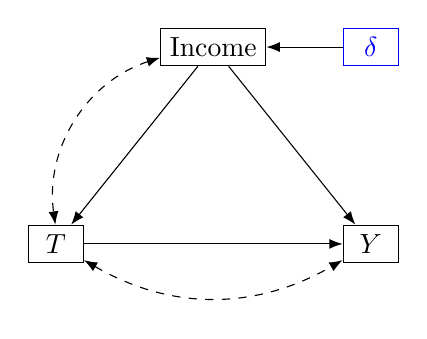
\begin{tikzpicture}
    \node[state, rectangle] (i) at (0,0) {Income};
       \node[state, blue, rectangle] (d) at (2,0) {$\delta$};
      \node[state, rectangle] (t) at (-2,-2.5) {$T$};
       \node[state, rectangle] (y) at (2, -2.5) {$Y$};
     
      \path (t) edge (y);
       \path (i) edge (t);
        \path (i) edge (y);
        \path (d) edge (i);
       \path[bidirected] (i) edge[bend left=-40] (t);
       \path[bidirected] (t) edge[bend left=-30] (y);
 

\end{tikzpicture}


  \clearpage
  
  
  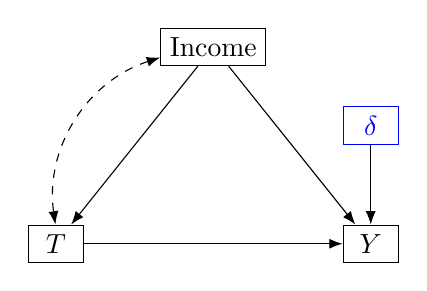
\begin{tikzpicture}
    \node[state, rectangle] (i) at (0,0) {Income};
       \node[state, blue, rectangle] (d) at (2,-1) {$\delta$};
      \node[state, rectangle] (t) at (-2,-2.5) {$T$};
       \node[state, rectangle] (y) at (2, -2.5) {$Y$};
     
      \path (t) edge (y);
       \path (i) edge (t);
        \path (i) edge (y);
        \path (d) edge (y);
       \path[bidirected] (i) edge[bend left=-40] (t);
      

\end{tikzpicture}

% (v, h)
  \clearpage
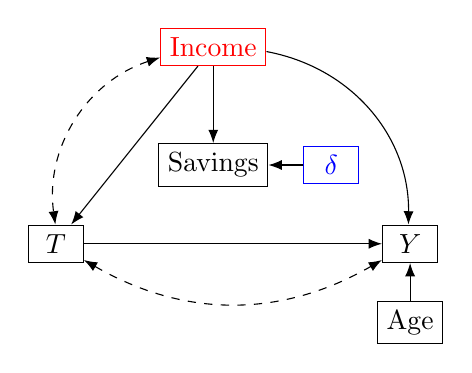
\begin{tikzpicture}


    \node[state, red, rectangle] (x1) at (0,0) {\text{Income}};
    
    \node[state, rectangle] (t) at (-2,-2.5) {$T$};
    
     \node[state, rectangle] (x2) at (0,-1.5) {\text{Savings}};
     
     \node[state, blue, rectangle] (d) at (1.5,-1.5) {$\delta$};
     
      \node[state, rectangle] (x3) at (2.5,-3.5) {\text{Age}};
      
      \node[state, rectangle] (y) at (2.5,-2.5) {$Y$};

      \path (x1) edge (t);
       \path (x1) edge (x2);
      \path (d) edge (x2);
       \path (x1) edge[bend left=40] (y);
       \path (x3) edge (y);
        \path (t) edge (y);
       \path[bidirected] (x1) edge[bend left=-40] (t);
       \path[bidirected] (t) edge[bend left=-30] (y);



\end{tikzpicture}
  

  \clearpage
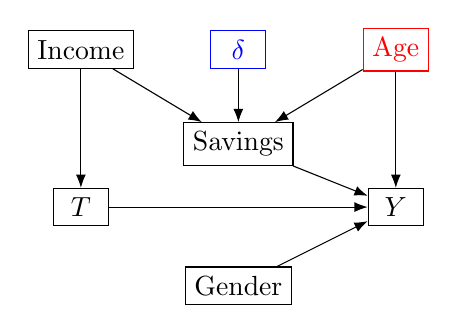
\begin{tikzpicture}

 % (v, h)
    \node[state, rectangle] (i) at (0,0) {\text{Income}};
     \node[state, rectangle] (t) at (0,-2) {\text{$T$}};
      \node[state, rectangle] (s) at (2,-1.2) {\text{Savings}};
      \node[state, red, rectangle] (a) at (4,0) {\text{Age}};   
      \node[state, rectangle] (y) at (4,-2) {$Y$};
       \node[state, blue, rectangle] (d) at (2,0) {$\delta$};
       \node[state, rectangle] (g) at (2,-3) {\text{Gender}};

     

      \path (i) edge (t);
        \path (t) edge (y);
        \path (i) edge (s);
         \path (d) edge (s);
          \path (a) edge (s);
           \path (s) edge (y);
           \path (a) edge (y);
        \path (g) edge (y);

  


\end{tikzpicture}
  



  



\end{document}